\documentclass[letterpaper]{article}
\usepackage[T1]{fontenc}
\usepackage{textcomp}
\usepackage{mathptmx}
\usepackage[scaled=0.9]{helvet}
\usepackage{url}
\usepackage{graphicx}
\setcounter{secnumdepth}{-2}
\title{Google Affiliate Network Plugin User Manual (V6)}
\author{Robert Heller}
\date{\today}
\begin{document}

\maketitle

\tableofcontents

\section{Introduction}

I wrote this plugin to display ads from the Google Affiliate Network on
Deepwoods Software's WordPress powered website. This plugin uses a
database of ads to display.  The ads are displayed in rotation, using
the simple method of counting ad impressions and giving priority to the
advertisers with the least impressions and display ads with the least
impressions first that are expiring soonest.  As ads and advertisers
are displayed, their impression counts are incremented, which moves
them down the list\footnote{To the back of the list once the impression
counts reach equilibrium, when the impression counts are all the
same.}.  This means that all ads are displayed fairly, with preference
given to new ads and to ads which are expiring soonest\footnote{Expired
ads are not displayed and a daily cron job deletes them.}. After using
``in house'' for a while, I have made this plugin available to other
WordPress users who also using the Google Affiliate Network as a source
of advertising revenue.

There are two type of ads: Link Ads, which are links to advertisers' web
pages and Product Ads, which are links to product buy pages.  Both kinds
of ad units are supported by the current version of this plug in.  The
ad information is different and the ads are kept in separate database
that are managed separately.

This manual has been updated for version 6.0 of the plugin, which is a
major re-write of the code.

\section{Installation}

Installation is just a matter of installing from the new plugin
page.  Once installed and activated, the plugin is ready to start
displaying affiliate ads.

\section{Configuring}

There are two configuration options: one for automatically deleting
expired ads and one to add additional CSS to fine tune how the ad
blocks look.  The option to automatically delete expired ads is on by
default. While it is possible to disable automatically deleting expired
ads it is not recommended.  The additional CSS section can be used to
adjust the look of ad blocks.  For the outer iframe, and for img and p
tags in the ad units, the class attribute is set to GANleader for
horizontal ad units and GANright for vertical ad units.  Within the ad
unit (link ads), there is a ul tag, whose id attribute is set to
GANleader for horizontal ad units and GANright for vertical ad units. 
You can use these CSS selectors:

\begin{description}
  \item[iframe.GANleader] For the outer iframe of horizontal ad units.
  \item[img.GANleader] For the product images of horizontal product ad units.
  \item[p.GANleader] For the product description of horizontal product ad
units.
  \item[ul\#GANleader] For the list of link ads in horizontal ad units.
  \item[iframe.GANright] For the outer iframe of vertical ad units.
  \item[img.GANright] For the product images of vertical product ad
units.
  \item[p.GANright] For the product description of vertical product ad
units.
  \item[ul\#GANright] For the list of link ads in vertical ad units.
\end{description}

The file, GAN.css in the css directory, is the default stylesheet.

If you have upgraded from an older version of the plugin, the
configure page will display a button to upgrade the database to the new
version.

\section{Managing your link ad database}

\begin{figure}[ht] \begin{centering}
\includegraphics[width=4.5in]{ganlinkads.png} 
\caption{GAN Link Ads Admin Page} 
\label{fig:ganlinkads} 
\end{centering} 
\end{figure} 
Managing your ads is done from the GAN Link Ads page, shown in
Figure~\ref{fig:ganlinkads}. The advertiser, link id, link name, image size,
start date, end date, and enabled flag are displayed in this table. Ads
are intially sorted by increasing end date, by default, but can also be sorted
by  Link ID, Link Name, Image Size, or Start Date.  It is possible to
filter the displayed ad by advertiser and/or ad size.  You can also
search by Link Name. There is a button to enable all ads and to delete
ads that have expired.  Ads can be deleted or have their enable flag
toggled in bulk.  Ads can be individually edited, viewed, deleted or
have their enable flags toggled.  You can also delete, disable, and
enable by merchant.

\subsection{Inserting Link Ads}

In order to display ads, you need to have some ads in your database.
There are two ways to insert ads: manually, one by one or in bulk from
a TSV (Tab Separated Value) or CSV (Comma Separated Value) file. Manual
insertion is done on the \emph{Add new (Link)} admin page and bulk insertion
is done on the \emph{Add new (links in) bulk} admin page.

\subsubsection{Add new link ad admin page (manual link insertion)}

\begin{figure}[ht]
\begin{centering}
\includegraphics[width=4.5in]{ganaddlinkad.png}
\caption{GAN Manual Add Link Ad Page}
\label{fig:ganaddlinkad}
\end{centering}
\end{figure}
This page, shown in Figure~\ref{fig:ganaddlinkad}, has a form for adding
(and editing and viewing) a single ad. Generally, this page is not
usually used, see Section~\ref{sect:addbulklinks} for adding ads in bulk.
The fields\footnote{These fields correspond to the column headings used
in the files sent as part of your E-Mailed Link Subscriptions.}
include: 

\begin{description}
  \item[Advertiser:] This is the advertiser's name.
  \item[Link ID:] This is the (unique) Link Id code. This ID value is
supplied by Google and uniquely identifies the ad.  Link IDs must be
unique and are prefixed by an uppercase ``J''.
  \item[Link Name:] This is the name of the link.  It is used as the
anchor text for text ads.
  \item[Merchandising Text:] This is some ad copy for the
link and is displayed with the ad link.
  \item[Alt Text:] This is the alternative text for image
ads.
  \item[Start Date:] The is the starting date, in the format yyyy-mm-dd
or m/d/yyyy. 
  \item[End Date:] This is the ending date, in the format yyyy-mm-dd or
m/d/yyyy. For ads with no ending date use a date far into the future,
like 2037-12-31.
  \item[Clickserver Link:] This is the tracking URL for the ad. 
  \item[ImageURL:] This is the URL of the ad image for image ads. 
  \item[ImageHeight:] This is the height of the image (0 for text ads). 
  \item[ImageWidth:] This is the width of the image (0 for text ads). 
  \item[LinkURL:] This is the Link URL.  This is the URL of the actual
page.
  \item[PromoType:] This is the type of promotion.
  \item[MerchantID:] This is the (unique) merchant id.  This value is
supplied by Google and is prefixed by a uppercase ``K''.
  \item[enabled?] This indicates whether the ad is enabled or
not. 
\end{description}

\subsubsection{Add new links in bulk admin page (bulk link insertion)}
\label{sect:addbulklinks}

\begin{figure}[ht]
\begin{centering}
\includegraphics[width=4.5in]{ganaddlinkbulk.png}
\caption{GAN Bulk Add Link Page}
\label{fig:ganaddlinkbulk}
\end{centering}
\end{figure}
\begin{figure}[ht]
\begin{centering}
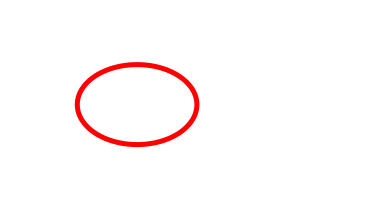
\includegraphics[width=2in]{ganLinksTab.png}
\caption{GAN Links Tab}
\label{fig:ganLinksTab}
\end{centering}
\end{figure}
\begin{figure}[ht]
\begin{centering}
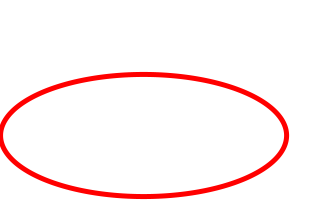
\includegraphics[width=2in]{ganExport.png}
\caption{GAN Export Links As}
\label{fig:ganExport}
\end{centering}
\end{figure}
This page, shown in Figure~\ref{fig:ganaddlinkbulk}, uploads a TSV or CSV file of ads
previously downloaded from your Google Affiliate Network management
page. You get this file by visiting your Google Affiliate Network
management page and clicking the Links tab (see
figure~\ref{fig:ganLinksTab}). On this page you can select the sorts of
ads you would like by selecting one or more of your approved
advertisers and selecting the type of ads (text and/or banner), and
other criteria such as size, etc. It is then possible to export these
ads as a TSV file, using the Export As button and selecting ``Tab
Separated Values'' option (see figure~\ref{fig:ganExport}), which can
then be downloaded. This same file can in turn be uploaded to the GAN
plugin and the ads in this file will be added to your ad database.

\subsection{Editing Ads}

When displaying the data on the main admin page, links are provided to
edit, delete, or toggle the enabled flag for each ad. It is possible to
select only a single merchant's ads to be displayed and/or a single
size of ad or only text ads.

\subsection{Link Subscriptions}

A Tcl script is included to process E-Mailed Link Subscriptions and
insert them into the database.  This requires the ability to receive
E-Mail on the server running the database server and requires that Tcl
and the MySQLTcl package be installed as well as the use of procmail as
a mail delivery agent.

\section{Managing your product ad database}

\begin{figure}[ht] \begin{centering}
\includegraphics[width=4.5in]{ganproducts.png}
\caption{GAN Products Admin Page}
\label{fig:ganproducts}
\end{centering}
\end{figure}

Managing your products is done from the GAN Product Database page,
shown in Figure~\ref{fig:ganproducts}. The advertiser, product name,
product brand, and enabled flag are displayed in this table. Products
are intially sorted by product name, but can be sorted by product brand
instead. It is possible to filter the displayed ad by advertiser. You
can also search by Product Name. There is a button to enable all
products. Products can be deleted or have their enable flag  
toggled in bulk.  Ads can be individually edited, viewed, deleted or  
have their enable flags toggled.  You can also delete, disable, and    
enable by merchant.

\subsection{Inserting Products}

In order to display products, you need to have some products in your
database. There are two ways to insert products: manually, one by one
or in bulk from a TSV (Tab Separated Value) or CSV (Comma Separated
Value) file. Manual insertion is done on the \emph{Add new (Product)}
admin page and bulk insertion is done on the \emph{Add new (Products
in) bulk} admin page.

\subsubsection{Add new Product admin page (manual product insertion)}

\begin{figure}[ht]
\begin{centering}
\includegraphics[width=4.5in]{ganaddproduct.png}
\caption{GAN Manual Add Product Page}
\label{fig:ganaddproduct}
\end{centering}
\end{figure}
This page, shown in Figure~\ref{fig:ganaddproduct}, has a form for adding
(and editing and viewing) a single product. Generally, this page is not
usually used, see Section~\ref{sect:addbulkproducts} for adding products
in bulk. The fields\footnote{These fields correspond to the column
headings in the TSV and CSV files generated by Google's product list
export.} include:

\begin{description}
  \item[Advertiser:] This is the advertiser's name.
  \item[Product Name:] This is the name of the product.
  \item[Product Description:] This is the description of the product.
  \item[Tracking URL:] This is the ``buy'' link for the product.
  \item[Creative URL:] This is the URL of the product's image.
  \item[Product Category:] This is the product's category.
  \item[Product Brand:] This is the product's brand.
  \item[Product UPC:] This is the product's UPC.
  \item[Price:] This is the product's price.
  \item[Merchant ID:] This is the advertiser id.
  \item[enabled?] This indicates whether the product is enabled or not.
\end{description}

\subsubsection{Add new products in bulk admin page (bulk product insertion)}
\label{sect:addbulkproducts}

\begin{figure}[ht]
\begin{centering}
\includegraphics[width=4.5in]{ganaddproductbulk.png}
\caption{GAN Bulk Add Product Page}
\label{fig:ganaddproductbulk}
\end{centering}
\end{figure}
\begin{figure}[ht]
\begin{centering}
\includegraphics[width=2in]{ganProductsTab.png}
\caption{GAN Products Tab}
\label{fig:ganProductsTab}
\end{centering}
\end{figure}
\begin{figure}[ht]
\begin{centering}
\includegraphics[width=2in]{ganExportProducts.png}
\caption{GAN Export Products}
\label{fig:ganExportProducts}
\end{centering}
\end{figure}
This page, shown in Figure~\ref{fig:ganaddproductbulk}, uploads a TSV
or CSV file of products previously downloaded from your Google Affiliate
Network management page. You get this file by visiting your Google
Affiliate Network management page and clicking the Products tab (see
figure~\ref{fig:ganProductsTab}). On this page you can search for
products that match a set of search terms. It is then possible to export
these ads as a TSV or CSV file, using the Export As button and selecting ``Tab
Separated Values'' option (see figure~\ref{fig:ganExportProducts}),
which can then be downloaded. This same file can in turn be uploaded to
the GAN plugin and the products in this file will be added to your product
database.

\section{Showing Ads}

There are two ways to show ads on your pages and/or posts.  You can use
one of the three widgets (GAN Image Widget (for image link ads), GAN
Widget (for text link ads), or GAN Product Widget (for product ads) or
one of the three shortcodes (GAN\_Text (for text link ads), GAN\_Image
(for image link ads), or GAN\_Product (for product ads)).  The widgets
of course need to go into a 'sidebar' that supports widgets.  The
shortcodes can go into any post or page.  They all generate an iframe
tag.

\subsection{GAN Widget}

\begin{figure}[ht]
\begin{centering}
\includegraphics[width=2in]{ganwidget.png}
\caption{GAN Widget}
\label{fig:ganwidget}
\end{centering}
\end{figure}
This widget (see Figure~\ref{fig:ganwidget}) shows text ads in a
``sidebar'' that supports widgets.

The GAN Widget has six parameters:
\begin{description}
  \item[Number of ads to display:] The number of ad links to display in
this ad unit.
  \item[Orientation:] The orientation of the ads. Horizontal
means the ads are arranged side by side like one row of a table and
vertical means the ads are arranged in a vertical list. Typically the
horizontal orientation is suitable for a wide but short ad frame and the
vertical orientation is suitable for sky scrapper type ad unit.
  \item[Advertisers:] The parameter can be used to limit the ad links to
a single advertiser.  The default is All, which is to use ads from all
advertisers.
  \item[Target:] The link target to use. Can be either Same 
Window or New Window or Tab.
  \item[Ad frame width:] The width of the ad frame. A value
of zero will cause the frame to use all of the available space.
  \item[Ad frame height:] The height of the ad frame.
\end{description}

\subsection{GAN Image Widget}

\begin{figure}[ht]
\begin{centering}
\includegraphics[width=2in]{ganimagewidget.png}
\caption{GAN Image Widget}
\label{fig:ganimagewidget}
\end{centering}
\end{figure}
This widget (see Figure~\ref{fig:ganimagewidget}) shows image (banner) 
ads in a ``sidebar'' that supports widgets.  Any given widget instance
(ad unit) can only show one size of banner ad.

The GAN Image Widget has eight parameters:
\begin{description}
  \item[Number of ads:] The number of ad links to display in
this ad unit.
  \item[Width:] The image width of the image ads.
  \item[Height:] The image height of the image ads.
  \item[Orientation:] The orientation of the ads. Horizontal
means the ads are arranged side by side like one row of a table and
vertical means the ads are arranged in a vertical list. Typically the
horizontal orientation is suitable for a wide but short ad frame and the
vertical orientation is suitable for sky scrapper type ad unit.
  \item[Advertisers:] The parameter can be used to limit the ad links to
a single advertiser.  The default is All, which is to use ads from all
advertisers.
  \item[Target:] The link target to use. Can be either Same 
Window or New Window or Tab.
  \item[Ad frame width:] The width of the ad frame. A value
of zero will cause the frame to use all of the available space.
  \item[Ad frame height:] The height of the ad frame.
\end{description}


\subsection{GAN Product Widget}

\begin{figure}[ht]
\begin{centering}
\includegraphics[width=2in]{ganproductwidget.png}
\caption{GAN Product Widget}
\label{fig:ganproductwidget}
\end{centering}
\end{figure}
This widget (see Figure~\ref{fig:ganproductwidget}) shows a product ad. 
Product ads contain an image of a product, with a link to the product
buy page.  There is generally a brief textual description of the product
and the product's price.

The GAN Product Widget has nine parameters:
\begin{description}
  \item[Orientation:] The orientation of the ads. Horizontal means the
product has the textual description to the right of the image and
vertical means the product has the textual description below the image.
Typically the horizontal orientation is suitable for a wide but short
ad frame and the vertical orientation is suitable for sky scrapper type
ad unit.  That is the vertical orientation is best in a narrow sidebar
and the horizontal orientation would be suitable for a `side bar' in the
wide part of the page (such as a side bar that is between posts or above
or below posts or page content).
  \item[Advertisers:] The parameter can be used to limit the product ads to
a single advertiser.  The default is All, which is to use products from all
advertisers.
  \item[Target:] The link target to use. Can be either Same 
Window or New Window or Tab.
  \item[Name Pattern:] This is a pattern that is matched to the product
name and if not empty will limit products to those that match this name.
  \item[Category Pattern:] This is a pattern that is matched to the
product category and if not empty will limit products to those that
match this category.
  \item[Brand Pattern:] This is a pattern that is matched to the product
brand and if not empty will limit products to those that match this brand.
  \item[Description Pattern:] This is a pattern that is matched to the
product description and if not empty will limit products to those that
match this description.
  \item[Ad frame width:] The width of the ad frame. A value
of zero will cause the frame to use all of the available space.
  \item[Ad frame height:] The height of the ad frame.
\end{description}


\subsection{GAN\_Text shortcode}

This shortcode inserts a text ad unit into a page or post.

The GAN\_Text shortcode has same six parameters as the GAN
Widget:
\begin{description}
  \item[maxads] An integer, with the default being 4.
The number of ads to display in this ad unit.
  \item[orientation] The orientation of the ads, one of
``vertical'' (the default) or ``horizontal''. Horizontal means the ads are
arranged side by side like one row of a table and      vertical means
the ads are arranged in a vertical list. Typically the horizontal
orientation is suitable for a wide but short ad frame and the vertical
orientation is suitable for sky scrapper type ad unit.
  \item[target] The link target to use, one of ``same'' (the
default) or ``new''.
  \item[ifwidth] The width of the ad frame. A value
of zero will cause the frame to use all of the available space.
  \item[ifheight] The height of the ad frame.
  \item[merchid] The advertiser id to limit ad links to.  An empty string
means use link ads from all advertisers.
\end{description}

Here is an example -- 5 text ads arranged horizontally in a 798x70 frame:
\begin{verbatim}
[GAN_Text maxads=5 orientation='horizontal' ifwidth=798 
ifheight=70]
\end{verbatim}

\subsection{GAN\_Image shortcode}

This shortcode inserts an image (banner) ad unit into a page or post.
Like the GAN Image Widget, all of the ads displayed are of the same
size. 

The GAN\_Image shortcode has same eight parameters as the GAN Image
Widget:
\begin{description}
  \item[maxads] An integer, with the default being 4.
The maximum number of ads to display in this ad unit.
  \item[orientation] The orientation of the ads, one of
``vertical'' (the default) or ``horizontal''. Horizontal means the ads are
arranged side by side like one row of a table and      vertical means
the ads are arranged in a vertical list. Typically the horizontal
orientation is suitable for a wide but short ad frame and the vertical
orientation is suitable for sky scrapper type ad unit.
  \item[target] The link target to use, one of ``same'' (the
default) or ``new''.
  \item[width] The image width of the image ads. The
default is 120.
  \item[height] The image height of the image ads. The
default is 60.
  \item[ifwidth] The width of the ad frame. A value
of zero will cause the frame to use all of the available space.
  \item[ifheight] The height of the ad frame.
  \item[merchid] The advertiser id to limit ad links to.  An empty string
means use link ads from all advertisers.
\end{description}

Here is an example -- 2 468x60 banners arranged vertically in a 468x126 frame:
\begin{verbatim}
[GAN_Image maxads=2 orientation='vertical' ifwidth=468 
ifheight=126 width=468 height=60]
\end{verbatim}

\subsection{GAN\_Product shortcode}

This shortcode inserts a product ad unit into a page or post. It is much
like the GAN Product Widget.

The GAN\_Product shortcode has same nine parameters as the GAN Product
Widget: 

\begin{description}
  \item[orientation] The orientation of the ads, one of ``vertical'' or
``horizontal'' (the default). The orientation of the ads. Horizontal
means the product has the textual description to the right of the image
and vertical means the product has the textual description below the
image. Typically the horizontal orientation is suitable for a wide but
short ad frame and the vertical orientation is suitable for sky
scrapper type ad unit.  That is the vertical orientation is best in a
narrow sidebar and the horizontal orientation would be suitable for a
`side bar' in the wide part of the page (such as a side bar that is
between posts or above or below posts or page content).
  \item[merchid] The parameter can be used to limit the product ads to
a single advertiser.  The default is '', which is to use products from all
advertisers.
  \item[target] The link target to use one of ``same'' (the
default) or ``new''.
  \item[namepat] This is a pattern that is matched to the product
name and if not empty will limit products to those that match this name.
  \item[catpat] This is a pattern that is matched to the
product category and if not empty will limit products to those that
match this category.
  \item[brandpat] This is a pattern that is matched to the product
brand and if not empty will limit products to those that match this brand.
  \item[descrpat] This is a pattern that is matched to the
product description and if not empty will limit products to those that
match this description.
  \item[ifwidth] The width of the ad frame. A value
of zero will cause the frame to use all of the available space.
  \item[ifheight] The height of the ad frame.
\end{description}

Here is an example -- a horizontal product ad the full with of the post
content column and 200 pixels high, limited to products with linux in
their description:
\begin{verbatim}
[GAN_Product orientation="horizontal" ifwidth="100%" 
ifheight="200" target="new" merchid="" namepat="" catpat="" 
brandpat="" descrpat="linux"]
\end{verbatim}

\subsection{Using the GAN ad unit insertion media button}

\begin{figure}[ht] 
\begin{centering}
\includegraphics[width=2in]{ganmediabutton.png} 
\caption{GAN Insert Ad Unit Media button} 
\label{fig:ganmediabutton} 
\end{centering}
\end{figure} 
\begin{figure}[ht] 
\begin{centering}
\includegraphics[width=4.5in]{ganinsertaddialog.png} 
\caption{GAN Insert Ad Unit Dialog Box} 
\label{fig:ganinsertaddialog}
\end{centering} 
\end{figure} 
As of version 4.3, a ``media button'', shown in
Figure~\ref{fig:ganmediabutton}, is available to aid in the insertion
of the ad unit short codes into pages and posts.  This button opens a
dialog window, shown in Figure~\ref{fig:ganinsertaddialog}, where the
parameters can be easily selected to create a short code that will
insert an ad unit (either for link ads or a product ad) into the
current page or post. You can select the maximum number of ads to
display in this ad unit, the size or type of ad, the orientation of the
ads within the ad unit and the size of the ad frame. When you click on
the insert ad button, the proper short code is generated and inserted
into your page or post.

\section{The ad rotation algorithm}

The ad rotation algorithm uses the impression count and the end date to
fairly display ads.  Impression counts are stored for each ad (links
and products) and each merchant.  When an ad from a given merchant is
displayed, that merchant's impression count is incremented.  And when a
given ad link or product is displayed, its impression count is
incremented.  These counts are used like this:

The ad display loop works like this:

First the merchant with the lowest impression count that has an ad of
the desired size is selected.  Then the ad from that merchant with the
lowest impression count, that also has the soonest end date is selected
(expired ads are not shown).  The HTML code for the ad is generated,
then the impression count for the ad and the merchant are incremented.
Then the process is repeated.  This means that every merchant gets a
shot and every ad of every merchant also gets a shot.

Some things to note:

If a merchant has a lot of ad links or products, each of these ad links
or products will be displayed fewer times than the ad links and
products of a merchant with a smaller number of ad links or products. 
Each merchant will get the same number of total impressions and these
impressions will be shared across all of the merchant's ad links or
products.  Ad links that will expire sooner will also get ``preferred''
exposure and will tend to get more impressions, at least until they
expire.  Newly added merchants,  ad links, and products will also get
``preferred'' exposure, since they will be starting with impression
counts of zero.  But over time, these ``new'' merchants and ads will
catch up with the older merchants ad links, and products.  It is
possible to zero the impression counts of merchants, ad links, and
products and this will ``level'' the playing field.

\section{Statistics}

Ad links, Products, and Merchant statistics are available for display
and download as CSV files.  The statistics are ordered from fewest
impressions to most impressions. A summary of the statistics is also
displayed on the dashboard.  Link Ad statistics can be filtered by
advertiser and/or by size. Product statistics can be filtered by
advertiser. It is possible to search Link Ad statistics and Product
statistics. 

In the statistics displays have the option to zero all, a select group,
or individual ads, products, or merchants. These impression counts are
used by the ad rotation algorithm.

\end{document}




